\chapter{Conclusions}

%appreciate the limitations of the methods employed and the results obtained by yourself and others
%understand how the broad conclusions of your thesis support, add to or conflict with previous work

% Sum up findings of four chapters

In my thesis I have analysed multiple RNA-seq datasets to uncover new insights into TDP-43 and FUS.
This work has explored the physiological roles of the two proteins in RNA regulation through loss-of-function experiments.
Furthermore, by using mutant mice as models of disease, I have uncovered mechanisms by which disease-associated mutations can impart a gain-of-function. 
This comparison between loss and gain of functionality will be crucial for understanding the onset and course of ALS/FTD.

In chapter 3 I developed software to discover and classify the full extent of cryptic splicing repression by TDP-43 and applied it to multiple mouse and human datasets.
I demonstrated that this repression is due to a combination of TDP-43 binding motifs and strong splice sites co-occurring within poorly conserved introns.
This mechanism was not seen in FUS knockdown, suggesting a divergence in function for the two proteins.
Later work has shown that cryptic exon repression is seen in a range of RNA-binding proteins, including the ALS associated MATRIN3, SFPQ and TIA1.

In chapter 4 I analysed data from a novel FUS mutant mouse which modelled aggressively early onset FUS ALS. 
By looking at two tissues and two time-points I identified a specific transcriptomic signature seen only in late-stage mouse spinal cord.
This was dominated by changes in mitochondrial and ribosomal genes.
Splicing changes at this tissue and time point were restricted to FUS itself and a small number of other genes including the myelin protein \textit{Mbp} and the FUS-interacting RNA-binding protein \textit{Ewsr1}.

In chapter 5 I compared two TDP-43 mutant mice, where one mutation caused a loss of splicing function due to the mutation affecting an RNA-recognition motif. 
The second mouse line had a mutation within the TDP-43 low complexity domain, the hotspot for ALS mutations.
I demonstrated that this mutation imparts a gain of splicing function, where instead of aberrant exon inclusion as seen in TDP-43 loss, there were a set of aberrant exon skipping events.
%I christened these events "skiptic exons" and showed that these affect constitutive exons and their skipping would more often than not lead to frame shifting and transcript degradation through nonsense-mediated decay. 
Some of these "skiptic" exons could be identified in TDP-43 mutant human patients.
I posit that the gain of splicing function could arise from a change in TDP-43 autoregulation.

In chapter 6 I compared three independent experiments where FUS was either knocked out or mutated to remove its nuclear localisation signal (NLS) in mouse neuronal tissues.
My joint analyses demonstrated significant overlap between the two FUS conditions in both gene expression and splicing, suggesting that FUS NLS mutations primarily deplete FUS from the nucleus.
Looking in detail at the FUS locus itself, I identified a novel mechanism by which FUS could regulate its own translation through intron retention. 
This autoregulation mechanism may be complementary to one previously reported exon skipping \citep{Zhou2013}.

All together, my results suggest specific consequences for loss of TDP-43 or FUS and gains of function in the cytoplasm, as seen in ALS/FTD.

\section{Issues arising from my work}

\subsection{Loss and gain of splicing function in TDP-43 and FUS}



% TDP loss leads to de-repression of cryptic exons
% these exons are not conserved between human and mouse - presumably due to lack of conservation of introns
% many alternate exons regulated by TDP are not conserved either or differ greatly in their change in response to TDP between human and mouse
% even within the same species they do not completely overlap between datasets
% each dataset has unique sets of exons
% This was seen in another study comparing TDP-43 deletion in mouse neurons, muscle cells and stem cells \citep{Jeong2017}.
% Each cell type will have a different set of RBPs expressed and binding to the same introns.
% the two human K562 cell datasets from ENCODE do not fully overlap despite being the same cell type
% some of this is probably technical due to polyA+ vs Total RNA
% but even the smaller list of total RNA cryptic exons are not merely a subset of the larger polyA + exons

Since I began studying TDP-43 and cryptic exons, many more RNA-binding proteins have been found to have a role in cryptic exon repression including PTBP1/2, RBM17, hNRNP L and MATR3 \citep{	Ling2016,Tan2016,McClory2018,Attig2018}. 
My own assessment of ENCODE knockdown data on a large number of RBPs showed that cryptic exon repression is a common feature seen in nearly all knockdowns with the exception of FUS (see chapter 3). 
% how important is loss of function to disease?

% multiple mouse models have shown that neurodegeneration can occur both without loss of TDP or FUS splicing function nor cytoplasmic aggregates.
% Mice are not humans

% Intron retention and complex splicing have been under-studied. 
% In chapter 5 I focussed on cassette exons due to the tractability of working with these splicing events. 
% But lots of information is lost.
% Complex events are subtle and hard to classify and may therefore be more prone to false positives.
% Intron retention is also highly dependent on library preparation. 
% In chapter 6 the polyA+ enriched FUS data (Dupuis) had very few detectable intron retention events compared to the other two total RNA datasets but this is also confounded by read length and depth.
% There may however be interesting biology in comparing intron retention via polyA+ and total RNA as the latter measures pre-mRNA as well as mature mRNA.
% Changes in total RNA intron retention may represent co-transcriptional changes whereas intron retention detected in polyA+ could be post-transcriptional splicing dynamics. 
% The FUS intron retention events are observed in both total and polyA+ libraries so is suggestive of the latter.

% RNA-binding proteins do not act alone.

\subsection{RNA-seq allows replication}

% Replication crisis - why most published results are probably false

% replication of the same phenonmenon in the same protein or model

% also, is a particular phenomenon common or specific to a particular protein?

% Both TDP-43 and FUS are linked to an every expanding list of roles within the cell, how many of these have been replicated?

% Open platform of RNA-seq, combined with data sharing and code sharing allows rapid replication to be done as standard.

% Caveats - particular phenomena may only be seen under certain experimental conditions or in particular cell types
% Example - circular RNA only seen with confidence when linear RNA are digested
% RNA is very dynamic. Very easy for batch effects to occur. Sequencing libraries prepared on different days and sequenced separately of the exact same cells or mice can show big differences.
% What is the fundamental observation? Correlating the expression or splicing of a gene with the expression of a protein, as in a knockdown study. 

\subsection{The value of annotation-free analysis}

Annotation initiatives have been successful in cataloguing genes and transcripts in many species.
They are very useful for any scientist interested in RNA biology by giving access to the genomic coordinates of a range of experimentally validated splicing isoforms.
There is however a danger in keeping too close to what annotation tells you.
There is great value in looking for things outside the framework given to you by annotation.

% use of annotation-free methods.
This is true for under-studied cell types such as  neurons which potentially harbour thousands of novel isoforms. %ref to that paper
In RNA biology, perturbing splicing by depleting particular factors could be expected to lead to unusual or aberrant splicing.
There is a need for tools that can robustly identify novel splicing events from sequencing data. 
In chapter 3 I developed such a tool, designed for use with low-quality RNA-seq data as it leveraged both read coverage and splice junctions.
Newer tools, as reviewed in chapter 2, depend on splice junctions alone, which are far more accurate but require high quality data.

Both cryptic exons and skiptic exons are examples of things that are not detected when not specifically looked for.
Yet both these phenomena could be widespread. 
Skiptic exons in particular could prove very rich to study due to their conservation between species. 
Unlike cryptic exons, constitutive exons are well-studied and defects in constitutive exon recogntion of the same exons by mutliple factors may be more apparent.

Further work on this may break down the current hard divisions between "constitutive" and "alternative" exons. This will require more work looking at "constititutive" splicing across mutiple tissues, such as the GTEX consortium. 



% protein level - big technical challenge and frontier
Going forward there is a pressing need to verify novel isoforms at the protein level. This will require new computational tools for shotgun mass spectrometry.
	
	
\section{Future directions for the work}

\subsection{Translating work into human patients}

It is regrettable that throughout my PhD I have not had the opportunity to explore more human RNA-seq samples and particularly those from human ALS/FTD patients.
The reason for this is partly due to scarcity of tissue but also the technical hurdles in analysis.
Unlike laboratory strains of mice, humans and highly heterogenous in both their genetics and the environmental exposures.
Even patients with identical mutations in a disease-associated gene could  expected to have many distinct modifying mutations as well as completely different life experiences.
Therefore any study on transcriptomics in humans would require much larger sample sizes to account for the increased variability in measurements of gene expression and splicing.
ALS/FTD patients would be expected to be particularly heterogenous due to the above genetic differences as well as variability in disease course and extent of pathology at death.

There are also technical considerations in sequencing post-mortem brains.
Both ALS/FTD patients and non-neurological control donor brains will often come from human patients who were kept on artificial respiration before death. 
This is known to affect RNA quality in post-mortem tissue due to changes in tissue pH.
This is the reason for most post-mortem tissue RNA-seq samples are prepared using total RNA libraries which may then dilute the amount of reads that will align to protein-coding genes of interest.

There are now large consortia established to collect and sequence large numbers of patient brains. 
As part of my post-doctoral studies I am looking forward to working with these consortia.

An alternative route for studying ALS/FTD in human brains is to grow patient neurons from induced pluripotent stem cells (iPSCs).
%These can be created from skin samples from patients and through a lengthy process, mature neurons can be created.

 neuronal organoids can be created. 
These can contain a variety of neuronal and glial cell types and replicate some basic topology of a human brain, with cells distributing to layers.


\subsection{Diving deeper into RNA regulation}

% bulk cell sequencing - need single cells
This work was all done with bulk cell short read RNA-seq. 
There are limitations to this approach that are both biological and technical.
Bulk RNA sequencing samples RNA from all cells in a population. 
This limits the observations that can be made to changes in expression and splicing that can be seen across a wide range of cells with low variability between cell types.
A rapidly developing solution to this is single-cell RNA sequencing, where individual cells are first separated from a tissue and sequencing libraries prepared using microfluidic technology.
Studies are now emerging of 10s of 1000s of individual cells being profiled. 
This has allowed for example an entire mouse brain to be classified into different cell types. %ref
The technology for this is still in its infancy and there is a problem with sequencing throughput to get enough reads per sample.
This will be important to overcome for analysing splicing changes due to the need for splice junction reads.
It would be very exciting if this technology could be applied to ALS/FTD patient brains. 

% need specific populations of RNA
Bulk sequencing also removes the distinction of RNA localisation within different cellular compartments. %distinction wrong word
For example, both FUS and TDP-43 bind transcripts in the cytoplasm and have some role in axonal transport. %ref
Fractionating RNA into nuclear or cytoplasmic would give information about nuclear retention of particular transcript, as I hypothesise for the FUS intron retention transcript identified in chapter 6.
Growing neurons in compartments as in \citep{Taliaferro2016} would allow specific populations of transcripts to be sequenced.
Alternatively, sequencing the nascently transcribed RNA would allow observation of unstable transcripts.
The nagging question from chapter 3 is that if I predict most cryptic exons to be degraded by NMD, why do I see any at all?
Silent splicing events were proposed in RBFOX proteins \citep{Jangi2014} to explain gene expression changes in RBFOX2-bound transripts without splicing changes.
If we were to sequence nascently transcribed RNA, perhaps with 4 thio-uridine, I could identify unstable transcripts that rapidly degrade upon export to the cytoplasm.
This may demonstrate cryptic splicing repression by TDP-43 to be much more widespread and why certain cryptic exon transcripts appear to evade NMD.



% problem with bulk sequencing
% lose cell-type specific information
%% single-cell RNA seq can do this
%% in disease brain one could select just cells with TDP or FUS pathology for analysis
% lose RNA localisation information
% some isoforms are preferentially transported - see Taliaferro
% Cytoplasmic NLS mutant FUS will play a role in transport - would need to fractionate

%Bulk cell or whole tissue sequencing means a loss of resolution
%RNA extracted from entire sections of tissue or populations of cells
% problem with short read sequencing
% cannot easily resolve complex transcripts
% evidence that some splicing events are co-regulated from Tilgner et al, need long reads to see this
% intron retention would be much simpler to detect
% still issues with throughput and error rate
Short reads






\section{Final thoughts}


% TDP but not FUS represses cryptic exons
% However cryptic exon repression can be seen in many RNA-binding proteins
% Repression of intronic sequences will be achieved by multiple proteins simultaneously
% "Crypic exons" that we see are just the tip of an iceberg, those sites where a single protein does most of the work
% Would explain low overlap between different knockouts in the same species
% Follow up paper showed lack of overlap between different mouse tissues

% TDP LCD mutations cause a gain of splicing function
% Inverse to cryptic exons, this is a role in maintaining canonical splicing that is being altered somehow by the mutation
% Suggests a spectrum between surveillance and maintenance functions
% Canonical splicing must be maintained and aberrant splicing must be repressed.
% TDP has roles in both
% It would be interesting to look through a range of RBPs and assess their skiptic and cryptic contributions - do they fit on a spectrum?
% Might expect proteins more deeply involved with the spliceosome to be more involved in supporting canonical exons than repressing
% Although one could also expect both functions depending on the position of binding, as are seen for alternate exons.

% FUS diverges from TDP, despite having shared roles in long intron genes, RNA transport and stress granules
% FUS does not repress cryptic exons, this could be due to weaker motif
% FUS KO and NLS mutations overlap, essentially both are loss of FUS function
% Splicing changes show few cassette exons and these are not enriched in iCLIP peaks.
% Excess of intron retention and complex events potentially an artefact of total RNA libraries, although the Dupuis dataset is polyA+ and contributes somewhat to splicing although less than the others.

% All the high quality mouse TDP data is polyA+ enriched so cannot make a fair comparison with the FUS knockout data.
% This loss of function is not seen in studying the delta 14 mice, as very few splicing events are seen.
% Gene expression profiles are completely different between embryonic HOM D14 and 12 month HET D14.
% The former shows neuronal and RNA binding terms, probably due to acute FUS loss
% Mitochondrial and ribosomal changes seen in 12 month D14 could be due to gain of function
% Other observations of FUS granules in the paper right?




% What does this mean for studying TDP and FUS?
% Two proteins have different functions
% They diverge on crypic exons



% What does this mean for ALS/FTD?
% Loss of RBP function is only one facet and it will be important to untangle these effects from a gain of function. The LCDmut shows that  without aggregation there is a specific effect on splicing, which can also be seen in human ALS patients


% What does this mean for RNA biology?



% What kind of work will follow this?










%\chapter{Next Steps for my PhD}
%
%My work so far has been on two very different projects centering around RNA regulation in models of ALS/FTD. The cryptic splicing project in TDP-43 was based on public data, which allowed for rapid progress and the ability to replicate my conclusions across multiple experiments. However, brute force knockdown of TDP-43 is a very crude model of disease and the project suffered from the low quality of RNA-seq data and the inability to validate the mechanism with a wet lab collaborator. The FUS $\Delta$14 mouse project however offers up a humanised mouse model where disease-like changes occur progressively. There is much appetite from Anny Devoy and from the lab of Pietro Fratta to continue investigations into the mechanism of the mutation's effect on RNA regulation.\\ 
%
%Over the remainder of my PhD I plan to upgrade the RNA-seq pipeline to use state-of-the-art splicing analysis software. I will then apply this pipeline to better understand the changes in splicing that occur in the FUS $\Delta$14 mouse, as well as in new data being generated on the mutation's impact on mRNA transport and translation. I will also apply the splicing pipeline to two opposing \textit{TARDBP} mutant mice and compare the results with existing TDP-43 knockdown data. To continue the cryptic splicing project I will screen the large ENCODE cohort of RNA-binding proteins for cryptic exon repression and then look for evidence of cryptic splicing in ALS/FTD patient brains. 
%	
%
%\section{Developing a full-featured splicing analysis pipeline}
%Since I started work on \textit{CryptEx} in October 2015 there have several major advancements in algorithms to analyse differential splicing from RNA-seq data. This has been enabled by improvement in the quality of RNA-seq data. \textit{CryptEx} and the underlying \textit{DEXSeq} approach were designed to work on all qualities of data going back to low depth, short read datasets generated in 2010. So while it has been useful for the TDP-43 project I believe I should make use of the state-of-the-art tools now available. Dr Kitty Lo and I have installed and assessed the latest advances in RNA-seq analysis algorithms. We can group software packages into one of four categories based on what they consider to be the fundamental unit of differential splicing. All of these modern algorithms require paired end data with high coverage and long reads to maximise the information available.
%
%\subsection{Transcript quantifiers}
%These compare abundances at the transcript level and rely on a curated list of known transcripts. Sequencing reads are then probabilistally assigned to a each transcript. This can be done extremely quickly in the case of pseudoaligners like \textit{Kallisto} \citep{Bray2015}. Transcript assembly algorithms like \textit{Stringtie} \citep{Pertea2015} can even assemble reads into novel transcripts. These algorithms require long reads for enough splicing information and very dependent on the list of transcripts they are given. Some genes can generate hundreds of very similar transcript isoforms or overlap with other genes and so these methods will struggle to accurately assign reads to them.
%
%\subsection{Exon quantifiers}
%These algorithms are typified by the \textit{DEXSeq} approach \citep{Anders2012}, where the transcripts are flattened to create a set of unique exon "bins".  As the bins themselves may not actually be an exon it makes the results difficult to interpret, although this has been lessened in a new software package called \textit{JunctionSeq} \citep{Hartley2015}, which also quantifies splice junctions and can pick up novel splice junctions. As they consider the whole gene they are sensitive to poorly annotated genes and extreme biases in coverage.
%
%\subsection{Local splicing event quantifiers}
%These algorithms work by comparing differences in splice junctions across the body of a gene while being agnostic to transcript annotations, allowing for the detection of novel events. These algorithms then establish different categories of possible events such as cassette exons, exon extensions, intron retention and alternate first or last exons. Each event is then tested for differences in inclusion/exclusion across conditions. This approach has been implemented in the \textit{SUPPA} \citep{Alamancos2015}, \textit{SGSeq} \citep{Goldstein2016} and \textit{MAJIQ} \citep{Vaquero-Garcia2016} packages. These packages, while providing a clear output of different splicing events, struggle to determine splicing events such as tandem 3'UTR changes which can only be differentiated by read coverage and not splice junctions. 
%
%\subsection{Annotation-free quantifiers}
%The fourth and final class of algorithm don't depend on any transcript annotation at all. The \textit{derFinder} package \citep{ColladoTorres2015} assesses changes in read coverage between samples, which is particularly useful in looking for novel non-coding RNA species or in the aforementioned tandem 3'UTR problem. The \textit{LeafCutter} package \citep{Li2016} looks for differentially used splice junctions independently of annotation and has shown that across a set of tissues around 30\% of the high confidence splice junctions recovered are novel to any annotation database.\\
%
%Dr Lo and I will create a pipeline that implements a combination of the above approaches to gain a full picture of splicing dysregulation in the FUS $\Delta$14 mouse and also in a different set of TDP-43 mutant mice.
%
%
%%%
%%%Stringtie is the successor to Cufflinks for assembling transcripts \citep{Pertea2015}.
%%%
%%%The DEXSeq methodology suffers from discarding the valuable information given by splice junctions and that has now been incorporated into the JunctionSeq package . 
%%%Categorising splicing changes
%%%SGSeq - what good for? \citep{Goldstein2016}
%%%SUPPA \citep{Alamancos2015}
%%%Annotation-free quantification of splicing derFinder \citep{ColladoTorres2015}
%%%LeafCutter \citep{Li2016}
%%%
%%%In collaboration with Dr Kitty Lo, we will build a state-of-the-art splicing pipeline.
%
%\section{RNA dysregulation in two opposing \textit{TARDBP} mutant mice}
%
%The lab of Dr Pietro Fratta have generated two mouse lines with mutations in TDP-43 from a large mutagenesis screen \citep{Ricketts2014}. One line, F210I, contains a mutation in the second RNA recognition motif and another, M323K contains a mutation in the C-terminal low complexity domain which is where the majority of ALS patient mutations occur \citep{Sreedharan2008-xv}. The F210I mutation is embryonic lethal in homozygosity whereas the M323K mutation appears to lead to a progressive motor neuron loss in adult mice. The Fratta lab has generated high quality RNA-seq data for the embryonic F210I and the adult M323K mice. Kitty Lo and I will apply our state-of-the-art splicing pipeline to investigate the splicing changes and compare them to existing TDP-43 knockdown data used in the cryptic splicing project. 
%Preliminary analysis has demonstrated a large number of cryptic exons in the F210I embryonic mice that overlap with the TDP-43 knockdown data from \citep{Polymenidou2011}. The lab has also generated iCLIP data by precipitating the RNA targets of the two mutant proteins (Dr Agnieszka Ule and Prasanth Sivakumar). It will be very interested to see how the two mutations alter TDP-43's splicing functionality and how that relates to toxicity and neurodegeneration.
%
%\section{Dissecting the role of FUS in mRNA transport and translation}
%The gene expression analysis of the FUS $\Delta$14 mice showed a general downregulation of ribosomal mRNAs. This is interesting as FUS has been noted to play a role in mRNA transport outside of the nucleus for local translation \citep{Kanai2004,Fujii2005} as well as modulating translation by transporting RNA to translationally active granules \citep{Yasuda2013} or to translationally silent stress granules \citep{Bosco2010}. In the light of this, the lab of Pietro Fratta want to observe the effect of the $\Delta$14 FUS mutation on both RNA transport in axons and the modulation of translation. 
%The impact of the FUS $\Delta$14 mutation on axonal transport will be observed by performing RNA-seq on spatially separated samples of motor neuron cell bodies and axons. This approach has been successful in wildtype neuronal cells \citep{Taliaferro2016}, where specific splicing isoforms were enriched in axons compared to cell bodies. This work will be carried out by Dr Nicol Birsa. I will process and analyse RNA-seq libraries created from both the axons and the cell bodies of wildtype and FUS $\Delta14$ motor neurons. I will try to compare axon-enriched mRNAs between wildtype and disease to uncover which mRNAs are affected by the FUS mutation, either by changes in localisation or changes in the splicing isoform for that gene.
%
%Polysome profiling involves immuno-tagging of a specific ribosomal protein in a specific cell type. These tagged ribosomes can be pulled down and the bound RNA can be sequenced to determine the RNA species and isoform \citep{Shigeoka2016}. This can then be compared to a background sequencing library to demonstrate an enrichment of a set of RNAs bound to ribosomes in mouse motor neurons carrying either the wildtype or mutant FUS. This work will be carried out by Dr Agnieszka Ule. I will then analyse RNA-seq libraries created from the ribosome-bound RNA to look for changes in translation between the wildtype and FUS $\Delta14$ motor neurons.
%
%By combining the two datasets I should be able to build a model of how the FUS $\Delta$14 mutations affects both the transport and translation of mRNAs. 
%
%\section{Screening the \textit{ENCODE} RNA-seq cohort for cryptic splicing}
%In chapter 3 I made use of publicly available RNA-seq data generated by the \textit{ENCODE} consortium (\url{www.encodeproject.com}) which has performed shRNA knockdown experiments on over 150 RNA-binding proteins, including the ALS/FTD-linked proteins TDP-43 and FUS, as well as MATR3, hnRNPA1, hnRNPA2B1 and TAF15. My cryptic splicing project concluded that TDP-43 but not FUS plays a role in repressing nonconserved elements of the genome from being included into transcripts but whether or not this occurs in other ALS-linked genes is unknown. There has not been a large screen of cryptic splicing across multiple proteins as previous studies have focussed on individual candidates: hnRNP C \citep{Zarnack2013-nv}, PTBP1/2 \citep{Ling2016} and RBM17 \citep{Tan07102016}.
%I therefore plan to download and align all shRNA knockdown data from ENCODE and run the data through both my own cryptic splicing pipeline (\textit{Cryptex}) and through a number of different algorithms that quantify novel splicing. I have already processed the data from the previously mentioned proteins and compared the number of high confidence cryptic exons discovered by \textit{Cryptex} with the strength of the knockdown of the target gene calculated by \textit{DESeq2} \citep{Love2014} (Figure 5.1). The results are promising as it appears that MATR3, TAF15 and hnRNPA2B1 knockdown leads to inclusion of a large number of cryptic exons, but only in experiments with a sufficiently strong knockdown. The results illustrate the variability in shRNA knockdown throughout the cohort. In TDP-43 around 70 cryptic exons can be seen in the K562 leukaemia cell line but fewer than 10 can be observed in the HepG2 liver carcinoma cell line, which has a much poorer knockdown. Screening the ENCODE cohort for cryptic splicing may uncover a new set of cryptic exon repressing RNA-binding proteins, or may even show that cryptic splicing repression is a common function of many RNA-binding proteins. 
%
%\begin{figure}
%	\begin{center}
%		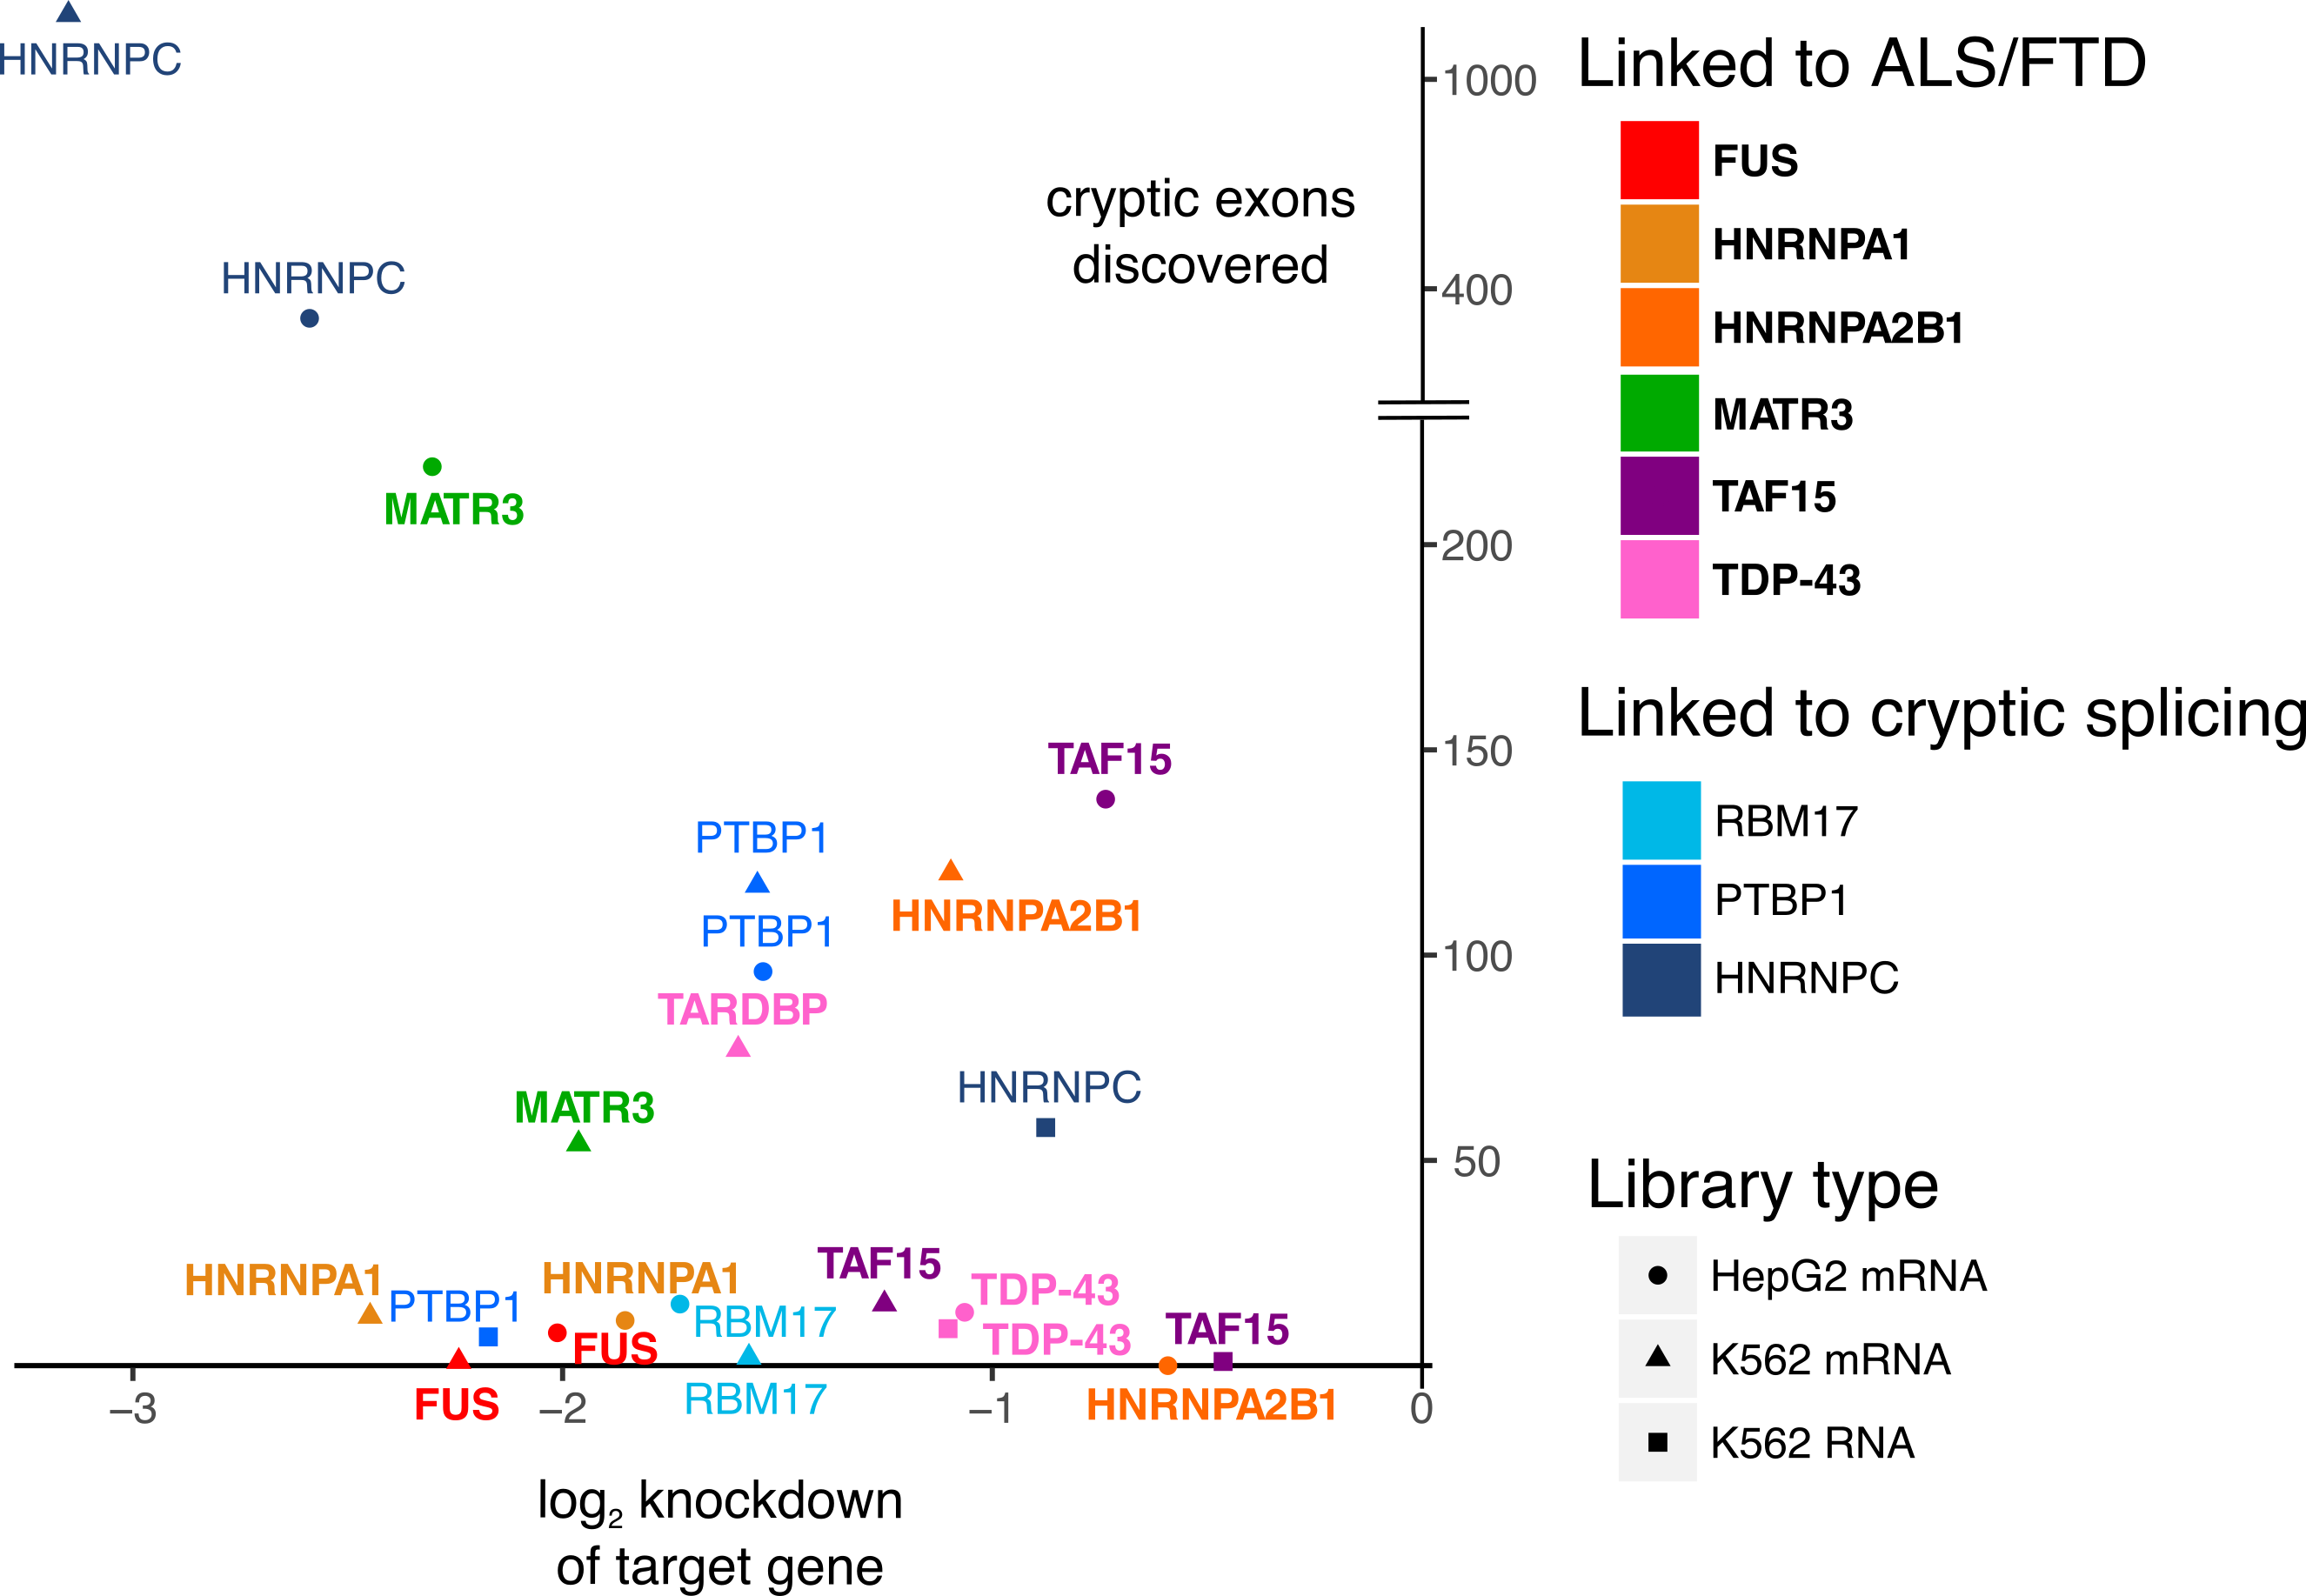
\includegraphics[width=12cm]{Figures/misc/ENCODE_summary.png}
%	\end{center}
%	\caption{ALS and cryptic splicing linked protein knockdowns from the ENCODE consortium  }
%\end{figure} 
%
%\section{Cryptic splicing in ALS and FTD patient brain}
%The initial paper on TDP-43 and cryptic splicing observed that two cryptic exons out of the 50 observed in HeLa cells could also be observed in the brains of ALS patients but not in non-neurological disease controls \citep{Ling2015}. Since then no further work has studied cryptic splicing in ALS or FTD brains. There are multiple lines of evidence that suggest that a number of RNA-binding proteins are perturbed in ALS/FTD as well as TDP-43 and FUS. Therefore if all the potential cryptic targets were known for a host of RNA binding proteins, the inclusion of these cryptic exons in diseased brain would suggest a perturbation in expression of that protein. 
%Building on the results of the TDP-43 cryptic splicing project and the results of the ENCODE screen, I want to thoroughly search for evidence of cryptic splicing in a set of control and disease brains. One such set of sporadic and familial ALS brain RNA-seq data has been previously published \citep{Prudencio2015}. We also have an in-house set of FTD and control brain RNA-seq (unpublished). The data will need to be very carefully prepared. I will attempt to deconvolute gene expression by cell type to compare the levels of neurons and glial cells in the control and diseased brains, to better understand differences in splicing changes between disease samples. RNA-seq of purified cells is available in mouse \citep{Newman2016} and algorithms for this specific task have been developed \citep{Zhang2014}. This approach has successfully applied to human brains to investigate cell type changes in aging \citep{Soreq2017}. There is also scope to look in patient blood and cerebrospinal fluid for potential RNA biomarkers to track disease course. 
%
%\section{Conclusions}
%My work so far has investigated RNA regulation in models of both sporadic and genetic ALS/FTD. Completion of my PhD should result in a fuller picture of cryptic splicing as a general mechanism of disease, complemented by a fine-grained analysis of specific mutations in \textit{TARDBP} and \textit{FUS}. Taking these insights into human patient tissue will be challenging but may lead to advances in understanding both ALS and FTD. 
%
